\chapter{Einführung}\label{ch:einführung}

Bei der Betrachtung dreidimensionaler Objekte in einem virtuellen Raum lässt sich deren Funktion häufig sofort erkennen. Ein Knopf soll gedrückt werden, ein Hebel soll sich bewegen, ein Display soll Informationen anzeigen und eine Lampe soll leuchten. Diese Funktionen sind von uns Menschen oft intuitiv aus Form, Position, Material und Kontext ableitbar. In virtuellen Umgebungen gilt dies jedoch nicht automatisch, da ein 3D-Modell zwar meist eine sichtbare Form, Materialien und räumliche Eigenschaften besitzt, aber in der Regel kein Verständnis über seine mögliche Nutzung. Auch Online-Bibliotheken, mittels 3D-Scanning erfasste Modelle realer Objekte sowie generativ erzeugte Inhalte liefern in der Regel kein Wissen darüber, welche Teile bedienbar sind oder wie diese auf Nutzer*innenhandlungen reagieren sollen. Zwischen dem visuellen Erscheinungsbild eines 3D-Objekts und seinem tatsächlichen Verhalten in einer virtuellen Welt liegt damit eine Lücke (siehe Abbildung~\ref{fig:intro_asset_examples}).

\begin{figure}[htbp]
    \centering
    \begin{subfigure}[b]{0.3\linewidth}
        \centering
        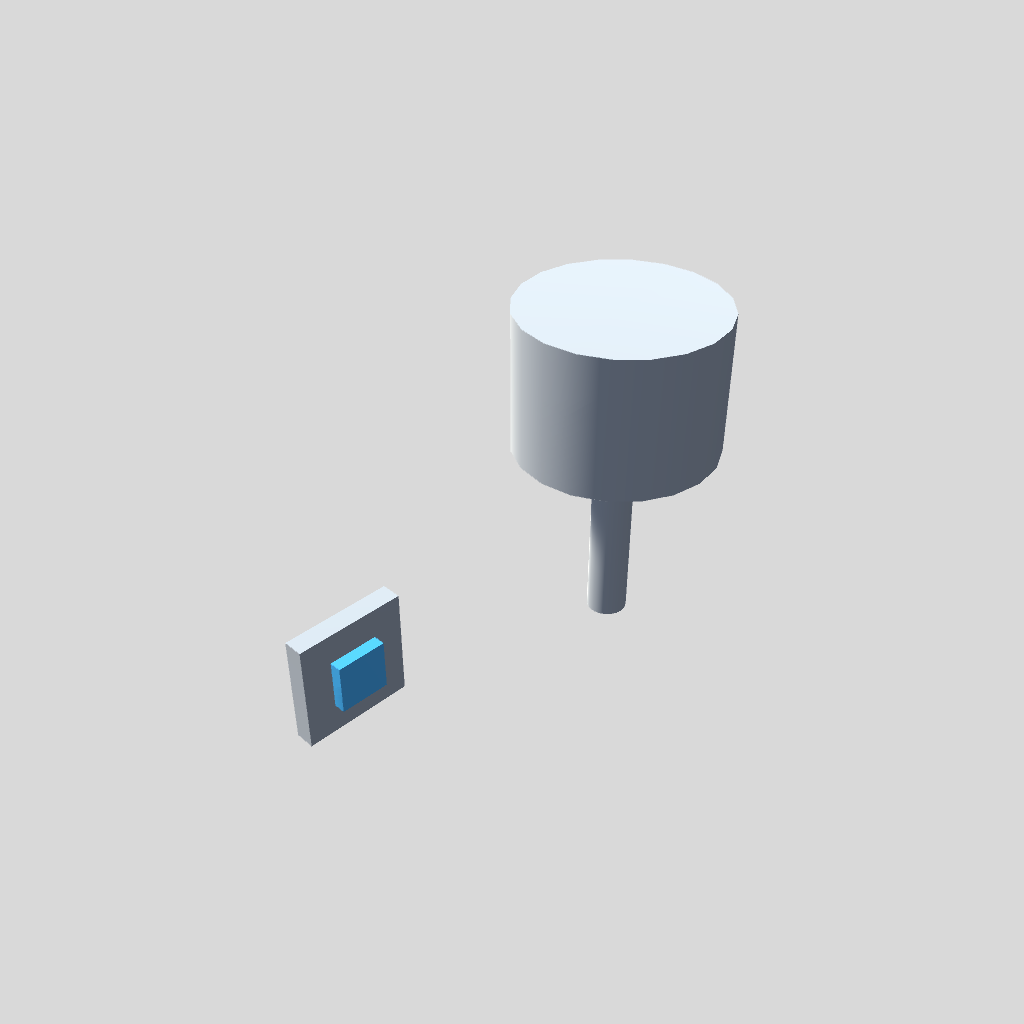
\includegraphics[width=\linewidth]{figures/asset-examples-iso/Lamp_iso_top_right}
        \caption{Lampe}
    \end{subfigure}\hfill
    \begin{subfigure}[b]{0.3\linewidth}
        \centering
        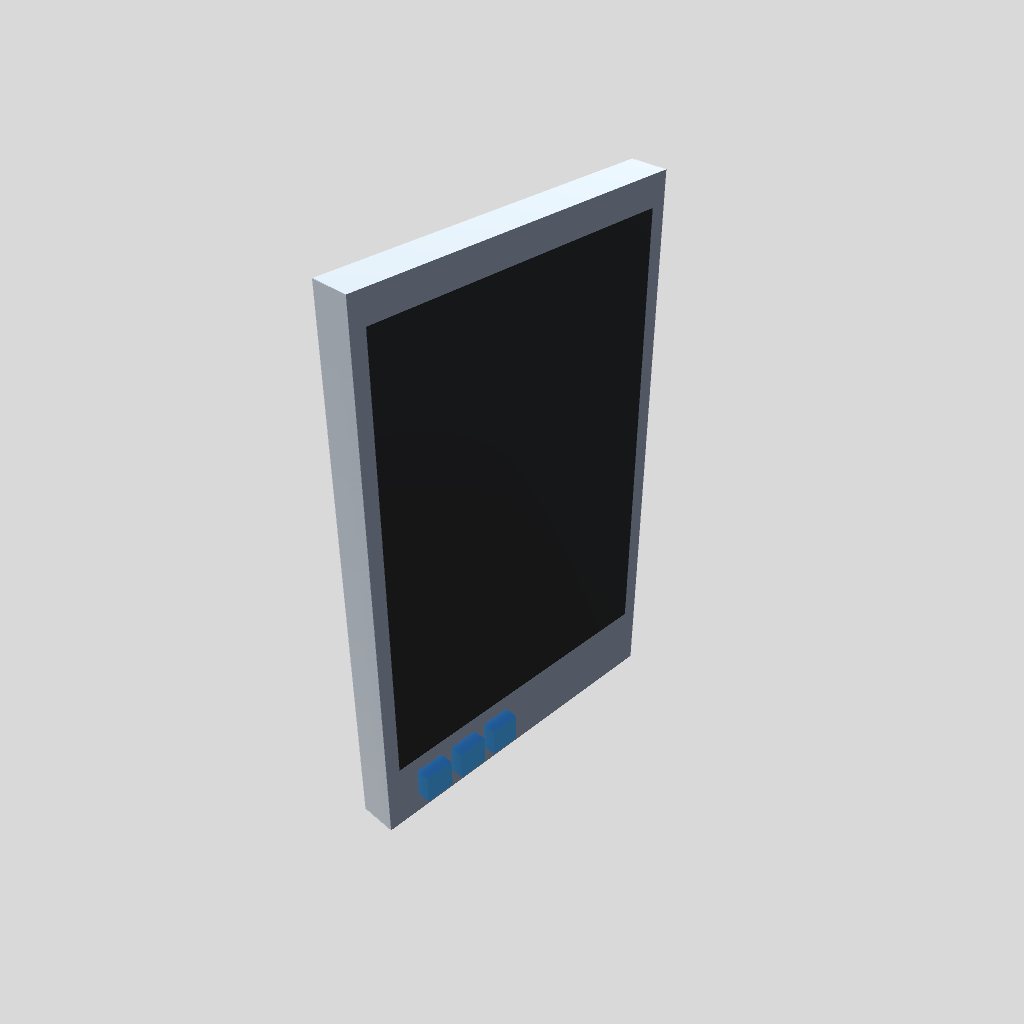
\includegraphics[width=\linewidth]{figures/asset-examples-iso/Display_iso_top_right}
        \caption{Display}
    \end{subfigure}\hfill
    \begin{subfigure}[b]{0.3\linewidth}
        \centering
        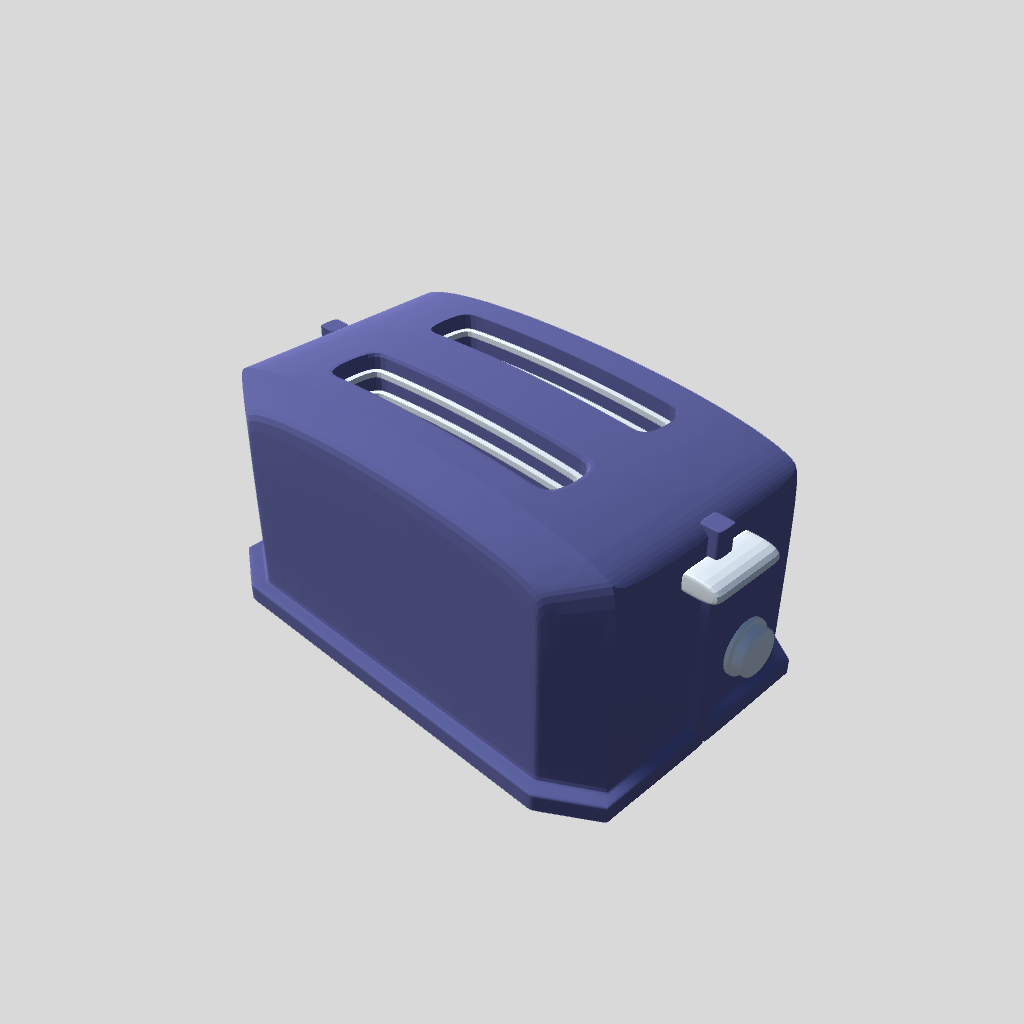
\includegraphics[width=\linewidth]{figures/asset-examples-iso/toaster3_iso_top_right}
        \caption{Toaster}
    \end{subfigure}
    \caption{Beispiele virtueller 3D-Objekte.}\label{fig:intro_asset_examples}
\end{figure}

Diese Lücke wird dann besonders deutlich, wenn 3D-Objekte nicht nur betrachtet, sondern als funktionale Prototypen mit bestimmtem Verhalten verwendet werden sollen. In Bereichen wie der Produktentwicklung, Lehre, \textit{Virtual Reality} oder \textit{Usability Engineering} reicht eine statische Darstellung häufig nicht aus, da Objekte ausprobiert, verändert und in ihrem Verhalten getestet werden sollen. Ein virtueller Prototyp muss damit weitaus mehr leisten als eine realistische Abbildung. Es muss Wissen darüber bestehen, welche Bestandteile relevant sind, welche davon bedienbar sind, welche Rückmeldungen gegeben werden und wie sich der Zustand des Objekts durch Interaktionen verändert.

Gleichzeitig ändert sich die Art und Weise, wie solche interaktiven Systeme entworfen werden können. Anstelle der rein manuellen Umsetzung durch Skripte oder systemspezifische Konfigurationen rückt mit der hohen Verfügbarkeit von KI-Systemen zunehmend natürliche Sprache in den Mittelpunkt. Diese wird somit zu einer Schnittstelle zwischen fachlicher Vorstellung und technischer Umsetzung. Der Fokus verschiebt sich von direkter Programmierung hin zur Beschreibung von Verhalten, Funktionen und Beziehungen.

Leistungsfähige \textit{Large Language Models} (LLMs) haben in den vergangenen Jahren eine rasante Entwicklung erfahren und können natürliche Eingaben interpretieren, semantische Zusammenhänge ableiten sowie strukturierte Ausgaben erzeugen~\cite{caffagniRevolutionMultimodalLarge2024,yinSurveyMultimodalLarge2024}. Dies eröffnet neue Möglichkeiten, die Lücke zwischen statischen 3D-Objekten und interaktiven Prototypen zu schließen, indem natürlichsprachliche Beschreibungen als Eingabe genutzt und mittels KI-gestützter Verfahren in eine maschinenlesbare Interaktionslogik übersetzt werden.

An dieser Stelle setzt die vorliegende Arbeit an. Sie untersucht, inwieweit sich bereits vorhandene statische 3D-Objekte in virtuellen Welten mithilfe eines KI-gestützten Workflows und natürlicher Sprache in interaktive virtuelle Prototypen überführen lassen. Als Grundlage dient das Vivian-Framework, welches Interaktion deklarativ über maschinenlesbare Spezifikationsdateien beschreibt. Damit bietet es eine geeignete Zielrepräsentation für eine automatisierte, durch Sprachmodelle gestützte Generierung.

\section{Problemstellung}\label{sec:problemstellung}

% Im Vivian Framework geschieht die Erstellung virtueller Prototypen deklarativ über Konfigurationsdateien für Interaktionselemente (InteractionElements), Visualisierungselemente (VisualizationElements), Zustände (States) und Übergänge (Transitions) in Verbindung mit einem statischen 3D-Modell. Obwohl dieses Vorgehen Interaktivität ohne tiefgreifende Programmierkenntnisse möglich macht, ist die manuelle Erstellung solcher Spezifikationen aufwendig sowie fehleranfällig. Es müssen sowohl die zulässigen Elementtypen, Attribute, Zustände, Events und Guards bekannt sein, als auch Namensreferenzen zwischen 3D-Szene und Spezifikation konsistent bleiben, da das Framework ein Verhalten über diese Referenzen an die Objekte einer 3D-Szene bindet.

% Mit steigender Komplexität eines Prototypen steigt diese Fehleranfälligkeit noch weiter. Dabei können diese syntaktischen, semantischen oder referenziellen Ursprungs sein und werden im Vivian Framework teils erst zur Laufzeit sichtbar.
% Um Spezifikationen automatisiert zu generieren, sind also formal gültige JSON-Strukturen allein nicht ausreichend. Inhaltlich plausible Interaktionen, korrekte Zustandsmodelle sowie konsistente Referenzen über mehrere Artefakte hinweg sind ebenfalls notwendig.
% Verwandte Arbeiten beschäftigen sich häufig mit Geometrie- oder Szenengenerierung, während

In der Regel enthalten statische 3D-Objekte Geometrie, Materialien und Transformationen, jedoch kein Wissen darüber, welche expliziten Teile bedienbar sind, welche Funktion sie erfüllen oder wie sie auf Nutzer*innenhandlungen reagieren. Für Interaktivität sind aber genau diese Informationen von fundamentaler Bedeutung, nämlich wenn Objekte oder Teilobjekte mit Bedeutung, möglichen Handlungen und Verhalten verbunden werden~\cite{kallmannModelingBehaviorsInteractive2002}.
Somit bestehen virtuelle, interaktive Prototypen nicht nur aus einer 3D-Geometrie, sondern besitzen zusätzlich semantisch-verhaltensbezogene Informationen.

Die Erstellung interaktiver 3D-Szenen oder die Transformation dieser in interaktive Prototypen setzt oft ein technisches Verständnis und Wissen voraus, wie etwa in 3D-Modellierung, Szenenaufbau oder Programmierung, was die Einstiegshürde für potenzielle Anwendende wie Produktentwickler*innen, Designer*innen oder Lehrende vergrößert. Diese Gruppe von Anwender*innen wird in dieser Arbeit als nicht-technische Benutzer*innen bezeichnet, also Personen ohne Kenntnisse in der Programmierung oder 3D-Modellierung. Die Fähigkeit, fachliche Anforderungen und Funktionalität präzise formulieren zu können, wird dabei jedoch vorausgesetzt.

Interaktivität wird meist an konkrete Objekte oder Teilobjekte gebunden. Verfahren wie 3D-Scanning erlauben allerdings häufig nur eine monolithische Erzeugung statischer Abbildungen der Realität. Auch rekonstruierte Szenen aus Punktwolken bieten an sich keine einzeln adressierbaren Teile. Diese Abbilder sind somit überwiegend nicht semantisch segmentiert und Objekte existieren nicht als eigenständige, adressierbare Entitäten. Eine interaktive Anpassung oder Segmentierung im Nachhinein ist dann nur mit massivem manuellem Aufwand möglich.

Weiterhin muss Interaktionsverhalten in eine konsistente, maschinenlesbare Repräsentation überführt werden, da interaktive Prototypen mehr als eine rein textuelle Beschreibung des gewünschten Verhaltens benötigen. Diese Überführung ist in der Regel ebenfalls mit hohem manuellem Aufwand verbunden und dadurch auch fehleranfällig.

Außerdem fehlen in automatisierten Verfahren zur Erstellung und Bearbeitung von virtuellen Prototypen oft interne Prüf- oder Korrekturmaßnahmen, um Fehler frühzeitig und im Prozess erkennen und beheben zu können. Diese Fehler müssen dann häufig zeitaufwendig und manuell im Nachhinein behoben werden. Auch können Halluzinationen auftreten, wie etwa in 3D-LLMs, wodurch Objekte teils nicht existieren oder falsche Beziehungen zwischen Objekten bestehen~\cite{pengUnderstandingEvaluatingHallucinations2025}.

Daraus lässt sich das zentrale Problem dieser Arbeit ableiten: Es fehlt ein niedrigschwelliger und dennoch kontrollierbarer Ansatz, mit dem bereits vorhandene statische 3D-Objekte in maschinenlesbare, validierbare und zustandsbasierte Prototypen überführt werden können, während die Geometrie beibehalten wird.


% Eine adressierte Problemstellung meiner Arbeit ist der manuelle Aufwand der Erstellung einer Vivian Spezifikation. Dies erfordert nicht nur Korrektheit der Werte sondern auch ein striktes Einhalten der benötigten Struktur.

% Eine adressierte Problemstellung meiner Arbeit ist die Planung der Einzelkomponenten, in der entschieden werden muss, welche Artefakte einer Spezifikation benötigt werden. Weiterhin muss das Wissen (Namen der Interaktionselemente, Zustände, etc.) über die einzelnen Teilartefakte zentral gespeichert werden, um darauf von verschiedenen Orten aus zuzugreifen. So kann Konsistenz der Daten über alle Artefakte hinweg gewährleistet werden.

% Da zur Erstellung einer Spezifikation für das Vivian Framework hinreichendes Wissen über dieses vorausgesetzt wird, ist ein weiteres Problem dieses Wissen einem System zu vermitteln. Es muss Kenntnis darüber besitzen, welche verschiedenen gültigen Werte und Bedingungen es für die einzelnen Artefakte zur Auswahl gibt.

% Da Fehler im Vivian Framework nativ erst zur Laufzeit geworfen werden und die Fehleranfälligkeit steigt, je komplexer das 3D-Asset ist, müssen Fehler bereits im Generierungsprozess sowie möglichst frühzeitig erkannt und abgefangen werden. Zudem ist zu berücksichtigen, ob es sich um semantische, syntaktische oder Referenzfehler handelt, damit sowohl fehlerfreie JSON-Strukturen, Gültigkeit der einzelnen Werte als auch Korrektheit der Referenzen sichergestellt werden kann. So kann außerdem ein Abbrechen des Systems verhindert werden, wenn Fehler im Generierungsprozess auftreten.


\section{Forschungsfragen und Zielsetzung}\label{sec:forschungsfragen_zielsetzung}

Um den in~\ref{sec:problemstellung} beschriebenen Problemen zu begegnen, untersucht die vorliegende Arbeit die Möglichkeit, einen Ansatz zu entwickeln, welcher die automatisierte Überführung statischer 3D-Objekte in validierte, zustandsbehaftete, interaktive Prototypen ermöglicht, der insbesondere auch nicht-technischen Benutzer*innengruppen eine Nutzung ermöglicht und die Geometrie der Teilobjekte beibehält.
Im Zentrum steht die folgende Forschungsfrage:



\begin{quote}
    \textbf{Lässt sich eine automatisierte Pipeline konzipieren und prototypisch umsetzen, die vorhandene statische 3D-Objekte mittels natürlicher Sprache in interaktive Prototypen überführt und dabei vorhandene Geometrien beibehält?}
\end{quote}

Zur detaillierten Beantwortung dieser Frage werden die folgenden untergliederten Forschungsfragen definiert:

\begin{itemize}
    \item \textbf{F1:} Lässt sich ein \textit{Co-Creation-Workflow} konzipieren und prototypisch umsetzen, in dem natürlichsprachliche Beschreibung und Korrekturschleifen die Überführung statischer 3D-Objekte in interaktive Prototypen unterstützen?
          %Kann ein Co-Creation-Workflow entworfen werden, der es auch nicht-technischen Benutzer*innengruppen ermöglicht, statische 3D-Objekte in interaktive Prototypen zu überführen?
    \item \textbf{F2:} Lassen sich relevante Objekte, Teilobjekte und semantische Rollen aus vorhandenen Szeneninformationen und Nutzer*innenbeschreibungen ableiten?
    \item \textbf{F3:} Können komplexe Interaktionslogiken aus der Kombination von bestehenden 3D-Geometrien und natürlicher Sprache extrahiert und in eine maschinenlesbare Repräsentation überführt werden?
    \item \textbf{F4:} In welchem Umfang tragen implementierte Validierungs- und Korrekturmechanismen dazu bei, aus fehlerhaften oder unvollständigen Erstgenerierungen lauffähige Vivian-Spezifikationen zu erzeugen?
          % In welchem Ausmaß reduzieren Validierungs- und Selbstkorrekturmaßnahmen syntaktische, semantische und referenzielle Fehler sowie fehlgeschlagene Unity-Validierungen im Vergleich zu einem Erstgenerierungsdurchlauf ohne Korrekturschleife?
          %Inwieweit können Validierungs- und Selbstkorrekturmechanismen bei der automatisierten Erstellung von Prototypen syntaktische, semantische und referenzielle Fehler vor der Laufzeit reduzieren?
\end{itemize}

Das Ziel dieser Arbeit ist die Konzeption und prototypische Implementierung einer KI-gestützten Pipeline, welche eine Überführung von statischen 3D-Objekten in interaktive Prototypen vornimmt und dabei natürliche Sprache entgegennimmt, um auch nicht-technischen Benutzer*innengruppen einen Zugang zu bieten. Dabei sollen die Fähigkeiten von LLMs genutzt werden und ein Co-Creation-Workflow entstehen, um einen Menschen in den Generierungsprozess einzubeziehen.

\section{Abgrenzung}\label{sec:abgrenzung}

Diese Arbeit ist in Kooperation mit dem Institut für angewandte Informatik (IFAI) der Technischen Hochschule Nürnberg Georg-Simon-Ohm entstanden. Aufgrund dieser Zusammenarbeit sowie der Expertise im Vivian Framework (siehe~\ref{sec:vivian_framework}), wurde dieses als Grundlage zur Umsetzung einer solchen Pipeline gewählt. Da dieses Framework interaktive Prototypen ausschließlich über eine maschinenlesbare Beschreibung des Verhaltens möglich macht, bietet es eine Basis, auf der LLM-gestützte Verfahren aufsetzen können.

Diese Arbeit zielt nicht darauf ab, 3D-Szenendaten oder Geometrie zu generieren. Das beinhaltet komplette 3D-Szenen sowie einzelne 3D-Objekte, wie es in einigen verwandten Arbeiten der Fall ist. Es wird ausschließlich die Spezifikationsableitung bereits vorhandener virtueller Szenen betrachtet, um virtuelle Prototypen durch Verwendung des Vivian Framework zu erschaffen.


\section{Aufbau der Arbeit}

Aufbauend auf den in Kapitel 1 genannten Problemstellungen und Forschungsfragen werden in Kapitel 2 einige theoretische Grundlagen erläutert. Dazu gehören statische und interaktive 3D-Objekte, die Transformation vorhandener 3D-Assets in interaktive Prototypen, das Vivian-Framework sowie Large Language Models und agentische Systeme. Kapitel 3 ordnet den derzeitigen Forschungsstand zur Verwendung von LLMs in virtuellen 3D-Welten ein und leitet daraus die Forschungslücke ab. Darauf aufbauend beschreibt Kapitel 4 die Anforderungen an den Vivian Specification Generator sowie Architekturentscheidungen. Kapitel 5 stellt die prototypische Implementierung der Pipeline und ihrer Module vor. In Kapitel 6 wird der entwickelte Ansatz anhand verschiedener Testassets technisch evaluiert und hinsichtlich Funktionsfähigkeit, Robustheit sowie Validierungs- und Korrekturmechanismen untersucht. Schließlich fasst Kapitel 7 die Ergebnisse der Arbeit zusammen, beantwortet die Forschungsfragen und zeigt Ansätze für mögliche weiterführende Arbeiten auf.